\begin{figure}[htbp]
    \centering
    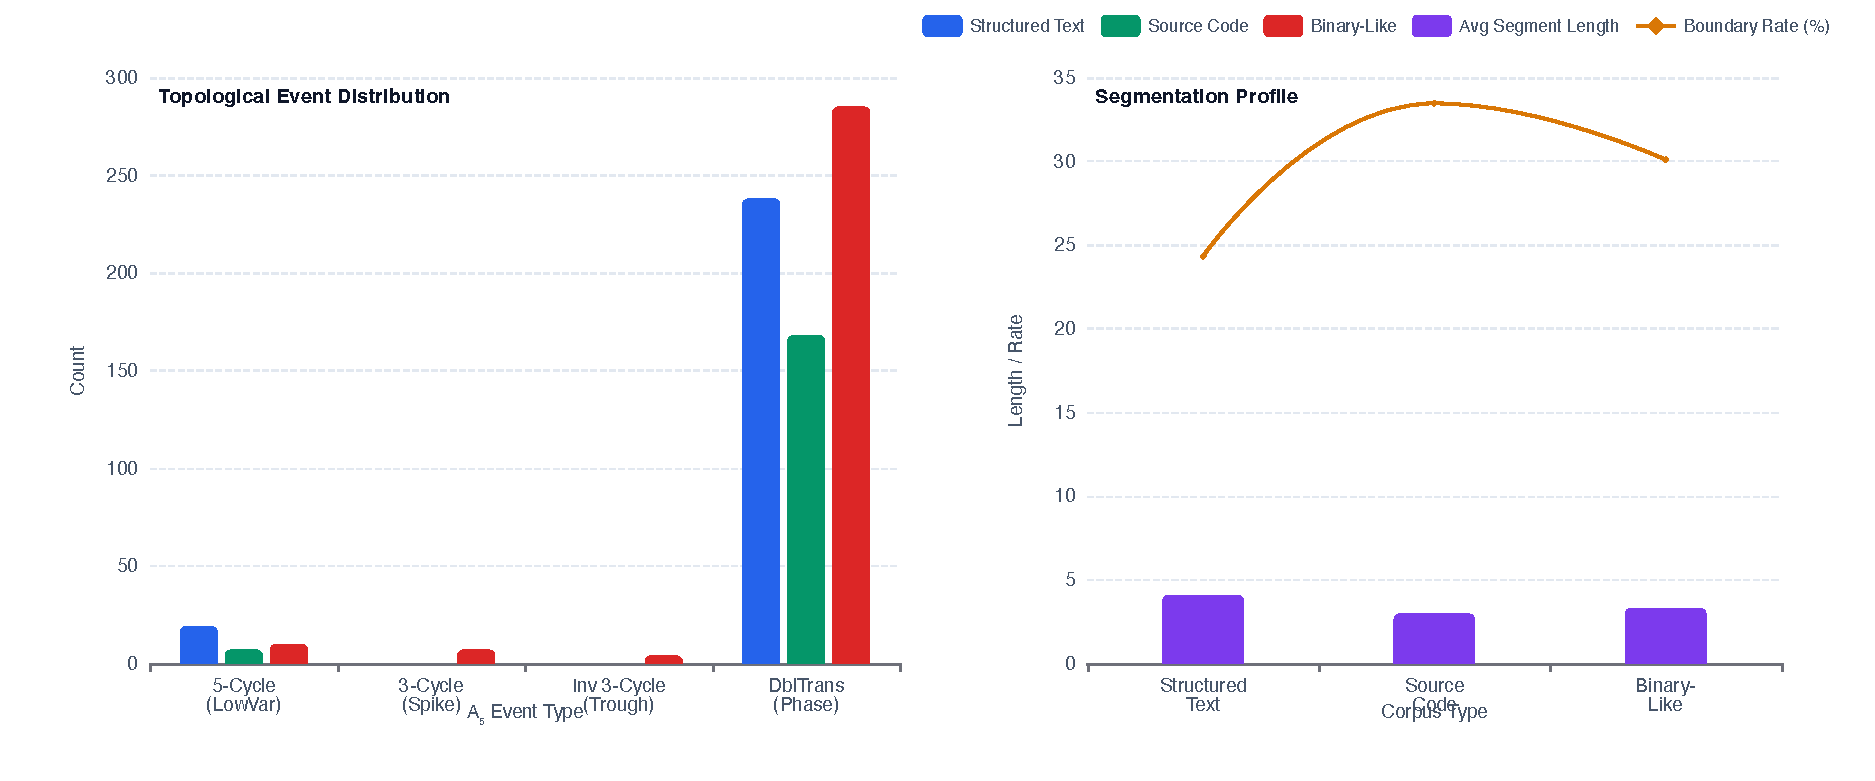
\includegraphics[width=1.0\textwidth]{sequencer_boundaries.pdf}
    \caption{(Left) Distribution of the four $A_5$ topological events across three corpus types. 5-Cycle (low variance flux) events dominate in all cases as the sequencer detects coherence saturation. 3-Cycle (density spike/trough) and Double-Transposition (phase inversion) events correlate with natural structural boundaries. (Right) Average segment length and boundary rate per corpus type. Structured text produces shorter, more frequent segments reflecting its natural sentence-level granularity.}
    \label{fig:sequencer_boundaries}
\end{figure}
